\documentclass[11pt]{article}

\usepackage{amsmath}
\usepackage{amsfonts}
\usepackage[margin=1in]{geometry}
\usepackage{enumitem}
\usepackage{graphicx}
\usepackage[colorlinks]{hyperref}
\usepackage{longtable}

\usepackage{helvet}
\renewcommand{\familydefault}{\sfdefault}

\setlength{\parindent}{0in}

\def\tightlist{}
\def\toprule{}
\def\bottomrule{}

\begin{document}

{\LARGE Homework 11 (Due December
9th)}\label{homework-11-due-december-9th}

{\Large 1. Coordinate Free Dipole
Equation}\label{coordinate-free-dipole-equation}

In class we derived the magnetic field formula for the magnetic moment
of a pure dipole which points in the z direction, located at the origin:

\[\mathbf{B} = \dfrac{\mu_0 m}{4 \pi r^3}(2 \cos \theta\,\hat{r} + \sin \theta\,\hat{\theta})\]

Here \(\mathbf{m}=I\mathbf{a}\) (\(\mathbf{a}\) is the area vector of
our tiny dipole) But sometimes \(\mathbf{m}\) points in another
direction than just \(z\)-hat! A more elegant way to write B which does
not explicitly depend on any choice of coordinate axes is:

\[\mathbf{B} = \dfrac{\mu_0}{4 \pi r^3}(3 (\mathbf{m}\cdot\hat{r})\hat{r} - \mathbf{m})\]

\begin{enumerate}
\def\labelenumi{\arabic{enumi}.}
\tightlist
\item
  For this problem, assume the second equation above is correct, define
  your \(z\)-axis to lie along the direction of the magnetic moment
  \(\mathbf{m}\), and show that this leads back to first equation.
\end{enumerate}

\emph{Coordinate free formulas are nice, because now you can find B for
more general situations!}

{\Large 2. Semi-classical electron dipole
moment}\label{semi-classical-electron-dipole-moment}

A thin uniform solid torus (a ``donut'') has total charge \(Q\), mass
\(M\). It rotates around its own central axis at angular frequency
\(\omega\), as shown.

\begin{figure}[htbp]
\centering
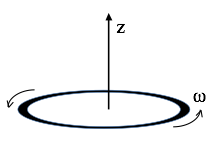
\includegraphics[width=2in]{./images/hw11/spinning_donut.png}
\end{figure}

\begin{enumerate}
\def\labelenumi{\arabic{enumi}.}
\tightlist
\item
  Find the magnetic dipole moment \(m\) of this rotating donut. What are
  the SI units of dipole moment?
\item
  Compute the ratio \(m/L\), the ``magnetic dipole moment'' divided by
  the angular momentum. This is called the ``gyromagnetic ratio''.
\item
  What is the gyromagnetic ratio for a uniform spinning sphere?
  \emph{HINT: This question really doesn't require any additional
  calculating: picture the sphere as a bunch of rings, and apply the
  result of part 2.}
\item
  In quantum mechanics, the angular momentum of a spinning electron is
  \(\hbar/2\). Use your results above to deduce the electron's magnetic
  dipole moment (in SI units.)
\end{enumerate}

\emph{Note: This ``semi-classical'' calculation is low by a factor of
almost exactly 2. Dirac developed a relativistic form of quantum
mechanics which got the factor of 2 right in the 1930's. In the '40's,
Feynman, Schwinger, and Tomonaga calculated tiny extra corrections
arising from QED (Quantum electrodynamics) For fun, find the current
best-value for the electron magnetic dipole moment. If you compare
theory and measurement, you will be extremely impressed at the agreement
(\textasciitilde{}12 digits!) It may make you ``believe'' in quantum
physics in a way you might not have before! That's not how it works in
practice though- people use this measurement to extract a fundamental
constant of nature, and then use that value to predict OTHER
experiments.}

{\Large 3. Force between magnets}\label{force-between-magnets}

Toy magnets seem to have a force law which ``turns on'' quite suddenly
as they approach, it doesn't really feel like a \(1/r^2\) force. That's
because it is not!

\begin{figure}[htbp]
\centering
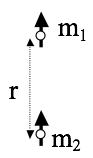
\includegraphics[width=1in]{./images/hw11/two_mag_dipoles.png}
\end{figure}

\begin{enumerate}
\def\labelenumi{\arabic{enumi}.}
\tightlist
\item
  Consider two small magnets (treat them as point-like perfect dipoles
  with magnetic moments \(m_1\) and \(m_2\), to keep life as simple as
  possible). In the configuration shown above (``opposite poles
  facing''), find the force between them as a function of distance r.
  (Does the sign work out for you sensibly?)
\item
  Let's do a crude estimate of the strength of the magnetic moment of a
  simple cheap magnet. Assume the atomic dipole moment of an iron atom
  is due to an (unpaired) electron spin. Question 2 above taught us what
  the magnetic dipole moment of a single electron is (or, just look it
  up to get the factor of 2 right!) The mass density and atomic mass of
  iron are also easy to look up. Consider a small, ordinary, kitchen
  fridge ``button sized'' magnet, and make a very rough estimate of its
  total magnetic moment.
\item
  Use your formula from part 1 to estimate how high (\(h\)) one such
  magnet would ``float'' above another (if oriented as shown below). 4.
  Does your answer seem at all realistic, based on your experiences with
  small magnets? (note that such a configuration is not stable - why
  not? I've seen toys like this, but they have a thin wooden peg to keep
  the magnets vertically aligned, that's how I drew it in the figure).
\end{enumerate}

\begin{figure}[htbp]
\centering
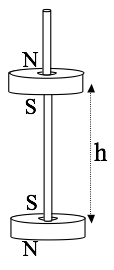
\includegraphics[width=1in]{./images/hw11/two_magnets.png}
\end{figure}

{\Large 4. Bound Currents I}\label{bound-currents-i}

Consider a long magnetic rod, radius \(a\). Imagine that we have set up
a permanent magnetization \(\mathbf{M}(s,\phi,z) = c \hat{z}\), with \(c\) =
constant. \emph{Neglect end effects, assume the cylinder is infinitely
long.}

\begin{enumerate}
\def\labelenumi{\arabic{enumi}.}
\tightlist
\item
  Calculate the bound currents \(\mathbf{K}_b\) and \(\mathbf{J}_b\) (on
  the surface, and interior of the rod respectively).\\
\item
  What are the units of \(c\)?
\item
  Use these bound currents to find the magnetic field inside and outside
  the cylinder. (Direction and magnitude)
\item
  Find the \(\mathbf{H}\) field inside and outside the cylinder, and
  verify that \(\oint \mathbf{H} \cdot d\mathbf{l} = I_{free}\) works.
  Explain briefly in words why your answer might be what it is.
\item
  Now relax the assumption that it is infinite - if this cylinder was
  finite in length (\(L\)), what changes? Sketch the magnetic field
  (inside and out). Briefly but clearly explain your reasoning. Please
  draw \emph{two} such sketches, one for the case that the length \(L\)
  is a few times bigger than a (long-ish rod, like a magnet you might
  play with from a toy set), and another for the case \(L \ll a\), which
  is more like a magnetic disk than a rod.
\end{enumerate}

{\Large 5. Bound Currents II}\label{bound-currents-ii}

Like the last question, consider a long magnetic rod, radius \(a\). This
time imagine that we can set up a permanent azimuthal magnetization
\(\mathbf{M}(s,\phi,z) = c s \hat{\phi}\), with \(c\) = constant, and
\(s\) is the usual cylindrical radial coordinate. Neglect end effects,
assume the cylinder is infinitely long.

\begin{enumerate}
\def\labelenumi{\arabic{enumi}.}
\tightlist
\item
  Calculate the bound currents \(\mathbf{K}_b\) and \(\mathbf{J}_b\) (on
  the surface, and interior of the rod respectively).
\item
  What are the units of \(c\)?
\item
  Use these bound currents to find the magnetic field \(\mathbf{B}\),
  and also the \(\mathbf{H}\) field, inside and outside. (Direction and
  magnitude)
\end{enumerate}

{\Large 6. Bound Currents III}\label{bound-currents-iii}

Once more, consider a very long cylinder (radius \(R\)) with a permanent
magnetization, this time again parallel to the axis:
\(\mathbf{M} = c s \hat{z}\), (where \(c\) is a constant, and \(s\) is
the usual distance from the cylinder's axis). There is no free current
anywhere.

\begin{enumerate}
\def\labelenumi{\arabic{enumi}.}
\tightlist
\item
  Find the magnetic field inside and outside the cylinder by figuring
  out the bound current everywhere and then figure out \(\mathbf{B}\)
  created by those.
\item
  Let's find the \(\mathbf{B}\) field inside and outside another way!
  This time, use Ampere's law in the form:
  \(\oint \mathbf{H} \cdot d\mathbf{l} = I_{free}\), and then use the
  standard relation,
  \(\mathbf{H} = \frac{1}{\mu_0}\mathbf{B} - \mathbf{M}\), to get
  \(\mathbf{B}\). (It should agree with part 1)
\end{enumerate}
\end{document}
